\documentclass[svgnames]{beamer}

\usepackage{preamble}
\usepackage{coursespecific}
%\renewcommand*{\IncludeAnswers}{1}

\renewcommand*{\Lecture}{14}
\subtitle{Introduction To Ajax}
\author{Ken Friis Larsen\\\scriptsize (Some slides prepared together
  with Henning Niss)}


\begin{document}

\begin{frame}
  \titlepage{}
\end{frame}


\begin{frame} 
\frametitle{Today's Script}
\begin{itemize}
\item Manipulating HTML pages through DOM
\item Ajax architecture
\item Intelligent clients
\end{itemize}
\end{frame}


\begin{frame}[fragile=singleslide] 
\frametitle{Setting The Style From JavaScript}

\begin{itemize}
\item To manipulate the CSS style on a DOM element from JavaScript, we
  use the \intro{\texttt{style}} property.
\begin{semiverbatim}
\footnotesize\color{gray}function validate_and_warn( s, warning_id ) \{
  var warning = document.getElementById(warning_id);
  if ( validate_int(s) ) \{
    \textcolor{black}{warning.style.visibility = "hidden";}
    return true;
  \} else \{
    \textcolor{black}{warning.style.visibility = "visible";}
    return false;
  \}\}
\end{semiverbatim}

\item Or, if we want to change the CSS class of a DOM element, we use
  the \intro{\texttt{className}} property
\begin{semiverbatim}
\footnotesize\color{gray}function zebra( table ) \{
  for ( var i = 0; i < table.rows.length; i++ ) \{
    if( i % 2 == 0 ) \{
      \textcolor{black}{table.rows[i].className = "oddrow";}
    \}
  \}\}
\end{semiverbatim}
\end{itemize}
\end{frame}

\begin{frame}[fragile=singleslide] 
\frametitle{Multiplication Table---Now With CSS}
\begin{tiny}
\begin{verbatim}
<html><head><title>Dynamic Multiplication Table With CSS Tricks</title>
<style type="text/css">
  .warning { ... ;  visibility: hidden; }
  .oddrow { background-color: silver; }
</style>
<script type="text/javascript" src="multcss.js" ></script>
<script type="text/javascript">
...
function inputchanged() {
  var cols = document.getElementById("cols");
  var rows = document.getElementById("rows");
  if ( cols.value != "" && rows.value != "" 
    && validate_and_warn(cols.value, "colswarning") 
    && validate_and_warn(rows.value, "rowswarning")) {   
     var tab = document.getElementById("multtab");
     clear_table( tab );
     add_multcells( tab, rows.value, cols.value );
     zebra( tab );
  }
}
</script></head>
<body> <h1>Dynamic Multiplication Table</h1>
  <form >
  Rows: <input type="text" name="rows" id="rows" onchange="inputchanged()" /> 
  <span id="rowswarning" class="warning">Number of rows must be an integer. 
  <img src="angry.png" /></span>
  <br />
  Columns: <input type="text" name="cols" id="cols" onchange="inputchanged()" />
  <span id="colswarning" class="warning">Number of columns must be an integer.
  <img src="angry.png" /></span>
  </form> 
  <table border="1px" id="multtab"></table>
</body></html>
\end{verbatim}
\end{tiny}
\end{frame}


\begin{frame}\frametitle{DOM Navigation}

  \begin{itemize}
  \item Navigation based on the id attribute or the tag name:
    \begin{itemize}
    \item \texttt{\textit{elem}.getElementById("i")}: get the child
      element with id \texttt{i}
    \item \texttt{\textit{elem}.getElementsByTagName("tag")}: get
      array of child elements with tag name \texttt{tag}
    \item (often we just use \texttt{document} as element)
    \end{itemize}

  \item Navigation based on a node (\texttt{n} is a node in the
    DOM tree):
    \begin{itemize}
    \item \texttt{n.parentNode}: parent of the node;
    \item \texttt{n.childNodes}: array of all children;
    \item \texttt{n.firstChild}: the first child;
    \item \texttt{n.lastChild}: the last child;
    \item \texttt{n.childNodes[i]}: the \texttt{i}'th child.
    \end{itemize}
  \end{itemize}
\end{frame}


\begin{frame}\frametitle{DOM Manipulation}

Adding children to a node (\texttt{n} is a node in the DOM tree):
\begin{itemize}
\item \texttt{n.appendChild(new)}: add a node after all children;
\item \texttt{n.insertBefore(new,old)}: add a node before a child;
\item \texttt{n.replaceChild(new,old)}: replace a child;
\item \texttt{n.removeChild(old)}: remove a child.
\end{itemize}

\medskip{}
Frames and Tables have special DOM methods for convenience. 
\end{frame}

\begin{frame}[fragile=singleslide] 
\frametitle{Shopping List With DOM}

\begin{scriptsize}
\begin{verbatim}
<html><head><title>Shopping Basket</title>
 <script type="text/javascript">
 function addToBasket() {
   var item = this;
   var li = item.parentNode;
   var ul = li.parentNode;
   var basket = document.getElementById("basket");
   basket.appendChild(item);
   item.onclick = null;
   ul.removeChild(li);
 }
 function addOnClicks() {
   var list = document.getElementById("list");
   var items = list.getElementsByTagName("li");
   for( var i = 0; i < items.length; i++) {
     items[i].firstChild.onclick = addToBasket;
   }}       
 </script>
 <body onload="addOnClicks()"><h1>Shopping List</h1>
  <ul id="list">
  <li><span id="beer">Beer</span></li> <li><span id="chips">Chips</span></li>
  <li><span id="fish">Fish</span></li> <li><span id="salted">Salted Peanuts</span></li></ul> <hr>
  <h1>Basket</h1>
  <div id="basket"></div> </body></html>
\end{verbatim}
\end{scriptsize}
  
\end{frame}




\begin{frame} 
\frametitle{Architecture---Now With Ajax}
\begin{itemize}[<+->]
\item The architecture until now
    \begin{tikzpicture}[thick,>=stealth]
    \footnotesize
    \fill[blue!25] (-1.5,-.8) rectangle (5.5,2.3);
    \path 
    (-5,2) node[draw,ellipse,minimum size=10mm](Client1) {Browser}
    (-5,0) node[draw,ellipse,minimum size=10mm](Client2) {Browser}
    (0,1.5) node[draw,rectangle,minimum size=10mm,fill=white,
                 text width=8em, text centered](WS) {Web Server\\(Apache)}
    (-.8,0) node[draw,rectangle,minimum size=10mm,fill=white,
                 text width=3em, text centered](PHP) {PHP file}
    (1,0) node[draw,rectangle,minimum size=10mm,fill=white,
                 text width=3em, text centered](HTML) {HTML file}
    (4,1.5) node[draw,rectangle,,minimum size=10mm,fill=white,
                 text width=8em, text centered](DB) {Database Server\\(MySQL)}
    ;
    \draw[<->] (Client1) -- node[above,sloped]{HTML/JavaScript}
                            node[below,sloped]{HTTP} (WS);
    \draw[<->] (Client2) -- node[above,sloped]{HTML/JavaScript} 
                            node[below,sloped]{HTTP} (WS);
    \draw[<->] (WS) -- node[above]{SQL} (DB);
    \draw[->] (PHP) -- (WS);
    \draw[->] (HTML) -- (WS);
    \end{tikzpicture}

  \item Ajax doesn't change the base architecture

    \begin{tikzpicture}[thick,>=stealth]
    \footnotesize
    \fill[blue!25] (-1.5,-.8) rectangle (5.5,2.3);
    \path 
    (-5,2) node[draw,ellipse,minimum size=10mm](Client1) {Browser}
    (-5,0) node[draw,ellipse,minimum size=10mm](Client2) {Browser}
    (-4.2,1.7) node[draw,fill=black!10,minimum size=1em](Ajax1) {Ajax}
    (-4.2,-0.3) node[draw,fill=black!10](Ajax2) {Ajax}
    (0,1.5) node[draw,rectangle,minimum size=10mm,fill=white,
                 text width=8em, text centered](WS) {Web Server\\(Apache)}
    (-.8,0) node[draw,rectangle,minimum size=10mm,fill=white,
                 text width=3em, text centered](PHP) {PHP file}
    (1,0) node[draw,rectangle,minimum size=10mm,fill=white,
                 text width=3em, text centered](HTML) {HTML file}
    (4,1.5) node[draw,rectangle,,minimum size=10mm,fill=white,
                 text width=8em, text centered](DB) {Database Server\\(MySQL)}
    ;
    \draw[<->] (Ajax1) -- node[above,sloped]{XML/Text}
                          node[below,sloped]{HTTP} (WS);
    \draw[<->] (Ajax2) -- node[above,sloped]{XML/Text} 
                          node[below,sloped]{HTTP} (WS);
    \draw[->] (Ajax1) |- ++(0,-.5) -| node[below,near start]{render} (Client1);
    \draw[->] (Ajax2) |- ++(0,-.5) -| node[below,near start]{render} (Client2);
    \draw[<->] (WS) -- node[above]{SQL} (DB);
    \draw[->] (PHP) -- (WS);
    \draw[->] (HTML) -- (WS);
    \end{tikzpicture}
\end{itemize}
  


\end{frame}



\begin{frame} 
\frametitle{What Is In A Name?}

\begin{uncoverenv}<+->
  \intro{Ajax} stands for \intro{A}synchronous \intro{J}avaScript
  \intro{A}nd \intro{X}ML.
\end{uncoverenv}

\begin{itemize}
\item<+-> Asynchronous??? \uncover<+->{What is asynchronous data retrieval?}
  \begin{uncoverenv}<+->
    \begin{itemize}
    \item also known as ``non-blocking'';
    \item send request, continue computing;
    \item when response ready, a callback function is called.
    \end{itemize}
  \end{uncoverenv}
\item<+-> OK, what is synchronous data retrieval then?
\begin{itemize}
\item also known as ``blocking'';
\item send request, wait for response;
\item when response is ready, continue computing.
\end{itemize}

\item<+-> Why would we want asynchronous data retrieval?
\begin{itemize}
\item proceed with useful things while waiting for response;
\item user can still work with the ``application'';
\item (potentially) many requests in parallel.
\end{itemize}
\end{itemize}
  
\end{frame}


\begin{frame} 
\frametitle{Synchronous}

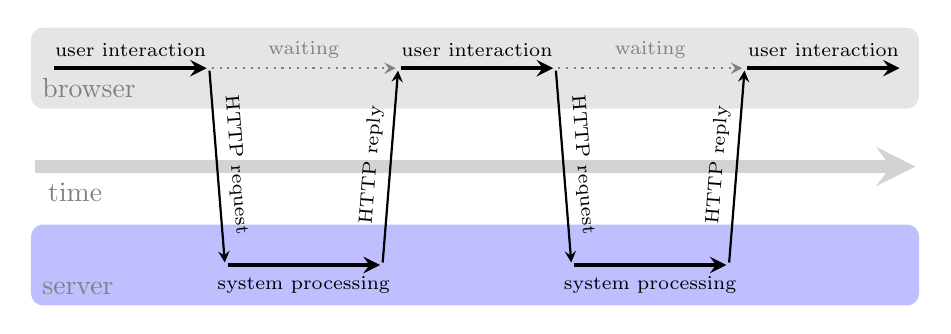
\begin{tikzpicture}[thick,>=stealth]
  \fill[draw,blue!25,text=black,rounded corners] 
    (-.25,-.5) node[above right] {\textcolor{gray}{server}} rectangle
    (11,.5)
  ;
  \fill[draw,black!10,rounded corners]
    (-.25,2) node[above right] {\textcolor{gray}{browser}} rectangle
    (11,3)
  ;
  \path [inner sep=0pt]
    (0,2.5) node (C1){}
    ++(2,0) node (C2){}
    ++(2.4,0) node (C3){}
    ++(2,0) node (C4){}
    ++(2.4,0) node (C5){}
    ++(2,0) node (C6){}
    (2.2,0) node (S1){}
    ++(2,0) node (S2){}
    ++(2.4,0) node (S3){}
    ++(2,0) node (S4){}
    (-.25,1.25) node (T1) {} 
    ++(11.25,0) node (T2) {}
  ;
  \draw[->,line width=5pt,LightGrey] 
       (T1) node[below right] {\textcolor{gray}{time}} -- (T2);
  \draw[->,ultra thick] (C1) 
        -- node[above] {\scriptsize{}user interaction} (C2);
  \draw[->] (C2) 
        -- node[above,sloped] {\scriptsize{}HTTP request} (S1);
  \draw[->,dotted,gray] (C2) 
        -- node[above,sloped] {\scriptsize{}waiting} (C3);
  \draw[->,ultra thick] (S1) 
        -- node[below] {\scriptsize{}system processing} (S2);
  \draw[->] (S2) 
        -- node[above,sloped] {\scriptsize{}HTTP reply} (C3);
  \draw[->,ultra thick] (C3) 
        -- node[above] {\scriptsize{}user interaction} (C4);
  \draw[->] (C4) 
        -- node[above,sloped] {\scriptsize{}HTTP request} (S3);
  \draw[->,dotted,gray] (C4) 
        -- node[above,sloped] {\scriptsize{}waiting} (C5);
  \draw[->,ultra thick] (S3) 
        -- node[below] {\scriptsize{}system processing} (S4);
  \draw[->] (S4) 
        -- node[above,sloped] {\scriptsize{}HTTP reply} (C5);
  \draw[->,ultra thick] (C5) 
        -- node[above] {\scriptsize{}user interaction} (C6);
\end{tikzpicture}
\end{frame}

\begin{frame} 
\frametitle{Asynchronous}

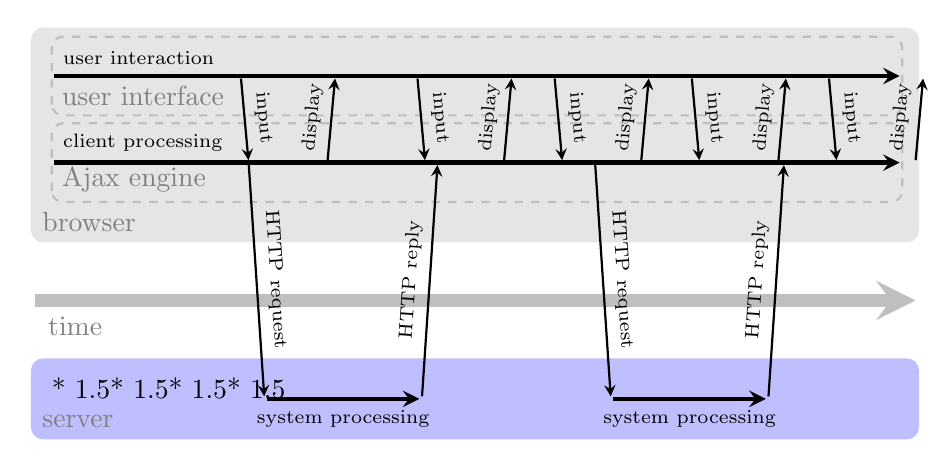
\begin{tikzpicture}[thick,>=stealth]
  \fill[draw,blue!25,text=black,rounded corners] 
    (-.25,-.5) node[above right] {\textcolor{gray}{server}} rectangle
    (11,.5)
  ;
  \fill[draw,black!10,rounded corners]
    (-.25,2) node[above right] {\textcolor{gray}{browser}} rectangle
    (11,4.7)
  ;
  \draw[lightgray,rounded corners,dashed]
    (0,3.6) node[above right] {\textcolor{gray}{user interface}} rectangle
    (10.8,4.6)
  ;
  \draw[lightgray,rounded corners,dashed]
    (0,2.5) node[above right] {\textcolor{gray}{Ajax engine}} rectangle
    (10.8,3.5)
  ;
  \path [inner sep=0pt]
    (0,4.1) node (U1){}
    +(10.8,0) node (UEND){}
    ++(2.4,0) node (U2){}
    ++(1.2,0) node (U2D){}

    (0,3) node (C1){}
    ++(2.5,0) node (C2){}
    +(1,0) node (C2D){}
    ++(2.4,0) node (C3){}
    ++(2,0) node (C4){}
    ++(2.4,0) node (C5){}
    ++(1.5,0) node (C6){}

    (2.7,0) node (S1){}
    ++(2,0) node (S2){}
    ++(2.4,0) node (S3){}
    ++(2,0) node (S4){}

    (-.25,1.25) node (T1) {} 
    ++(11.25,0) node (T2) {}
  ;
  \draw[->,line width=5pt,lightgray] 
       (T1) node[below right] {\textcolor{gray}{time}} -- (T2);
  \draw[->,ultra thick] (U1) 
       node[above right] {\scriptsize{}user interaction} -- (UEND);
  \draw[->,ultra thick] (C1) 
       node[above right] {\scriptsize{}client processing} -- (C6);
  \draw[->] (U2) 
        -- node[above,sloped] {\scriptsize{}input} (C2);
  \draw[->] (C2) 
        -- node[above,sloped] {\scriptsize{}HTTP request} (S1);
  \draw[->] (C2D) 
        -- node[above,sloped] {\scriptsize{}display} (U2D);
  \draw[->,ultra thick] (S1) 
        -- node[below] {\scriptsize{}system processing} (S2);
  \draw[->] (S2) 
        -- node[above,sloped] {\scriptsize{}HTTP reply} (C3);
  \draw[->] (C4) 
        -- node[above,sloped] {\scriptsize{}HTTP request} (S3);
  \draw[->,ultra thick] (S3) 
        -- node[below] {\scriptsize{}system processing} (S4);
  \draw[->] (S4) 
        -- node[above,sloped] {\scriptsize{}HTTP reply} (C5);

  \newlength{\temp}
  \foreach \i in {0,...,3} {
    \setlength{\temp}{\i cm * \real{1.5}} 
    \path[inner sep=0pt]
     ([shift={(\temp,0pt)}] U2D)
      ++(.3,0) node (UIA1\i){}
      ++(.1,-1.1) node (UIA2\i){}
      ++(1,0) node (UIA3\i){}
      ++(.1,1.1) node (UIA4\i){}
    ;
    \draw[->] (UIA1\i) 
          -- node[above,sloped] {\scriptsize{}input} (UIA2\i);
    \draw[->] (UIA3\i) 
          -- node[above,sloped] {\scriptsize{}display} (UIA4\i);
  };
\end{tikzpicture}
  \end{frame}


\begin{frame}
\frametitle{Client-side vs Server-side}

Not all reponses to user actions involves server:
\begin{itemize}
\item server not involved:
  \begin{itemize}
  \item data validation for user assistance;
  \item data editing in memory;
  \item (simple) navigation.
  \end{itemize}

\item server involved:
  \begin{itemize}
  \item data submitted for processing;
  \item loading interface code;
  \item retrieving new data.
  \end{itemize}
\end{itemize}
\end{frame}


\begin{frame}\frametitle{Better Use Of Resources}

Why move computation to the client?
\begin{itemize}
\item make clients more ``intelligent'';
\item better use of resources;
\item some resources server-side, some client-side;
\item client-side rendering;
\item server-side processing.
\end{itemize}
\end{frame}


\begin{frame}
\frametitle{Asynchronous HTTP Requests}

  \begin{itemize}
  \item Asynchronous requests programming is just like the event-based
    GUI programming. 
  \item A built-in JavaScript object allows us to make HTTP requests:
    \begin{itemize}
    \item \intro{\texttt{XMLHttpRequest}};
    \item supports synchronous and asynchronous requests;
    \item phases:
      \begin{enumerate}
      \item create instance
      \item open connection
      \item send request
      \item receiveresponse (later?)
      \end{enumerate}
    \item caveat: only requests to the host containing the script.
    \end{itemize}
  \end{itemize}
\end{frame}

\begin{frame}[fragile]
\frametitle{Making A Request}

\begin{semiverbatim}\footnotesize
function createRequest() \{
  var request = null;
  try \{ \textbf{request = new XMLHttpRequest();} \} catch (e) \{ 
  try \{ request = new ActiveXObject("Msxml2.XMLHTTP"); \} catch (e) \{ 
  try \{ request = new ActiveXObject("Microsoft.XMLHTTP"); \}
  catch (allHopeIsGone) \{
    if (request == null) \{
      alert("Error creating request object! Bad things will happen.");
    \}  
  \}\}\}
  return request;
\}
function sendRequest(requester,url,callback) \{
  \textbf{requester.onreadystatechange = function() \{
    callback(requester);
  \};
  requester.open("GET",url,true);
  requester.send(null);}
\}
\end{semiverbatim}
\end{frame}

\begin{frame}[fragile]\frametitle{Receiving A Reponse---Callbacks}

\begin{semiverbatim}\footnotesize
function receiveResponse(requester) \{
  if(\textbf{requester.readyState == 4}) \{ /* 4: response data available */
    if(\textbf{requester.status == 200}) \{ /* 200: HTTP OK */
      /* do something with the response;
         \textbf{requester.responseText} and \textbf{requester.responseXML}
      */
    \} else \{
      alert("Server returned " + requester.status);
    \}
  \}
\}
\end{semiverbatim}

\end{frame}


\begin{frame}[fragile] 
\frametitle{Example: Getting Course Evaluation Data}

\footnotesize
\begin{verbatim}
function showdata( textdata ) {
   var data = textdata.split(",");
   showdatatable( data );
}
function getquestion() {
   set_updatestatus();
   var selected = document.getElementById("questions").value;
   var xhr = createRequest();
   xhr.onreadystatechange = function() {
       if( xhr.readyState == 4 ) {
          if( xhr.status == 200 ) {
            showdata(xhr.responseText);
          } else {
            alert("The server returned "+ xhr.status +" for "+ selected);
          }
       }
     };
   xhr.open("GET","courseeval.php?question="+selected,true);
   xhr.send(null);
}
\end{verbatim}
  
\end{frame}


\end{document}

%%% Local Variables: 
%%% mode: latex
%%% TeX-master: t
%%% End: 
